\subsection{Captura 3 - Laboratorios del DC de FCEN-UBA}

Esta captura fue realiza en los laboratorios del Departamento de Computación de la FCEN. La captura duro veinte minutos, durante los cuales se capturaron $31632$ paquetes, de los cuales $4889$ fueron paquetes ARP.

\begin{figure}[H]
  \centering
    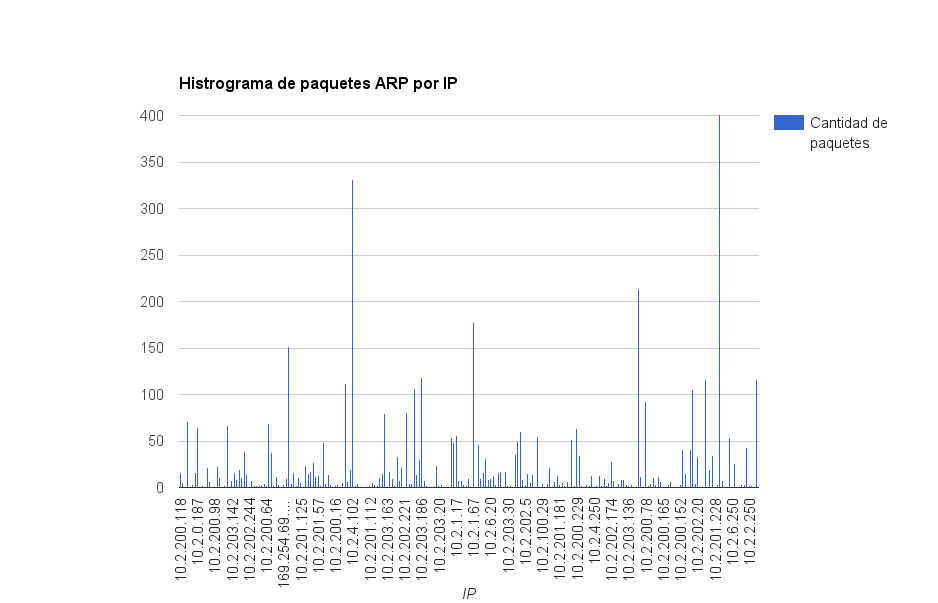
\includegraphics[width=1.1\textwidth]{imagenes/labosDC/histograma.png}
  \caption{Histograma de los símbolos de la fuente $S_1$}
  \label{fig:ejemplo}
\end{figure}

Esta red es la primera que presenta dos nodos con una frecuencia alta. El de mayor frecuencia probablemente sea el router pero no sabemos qué causa que otro nodo también cuente con una frecuencia tan alta.

\begin{figure}[H]
  \centering
    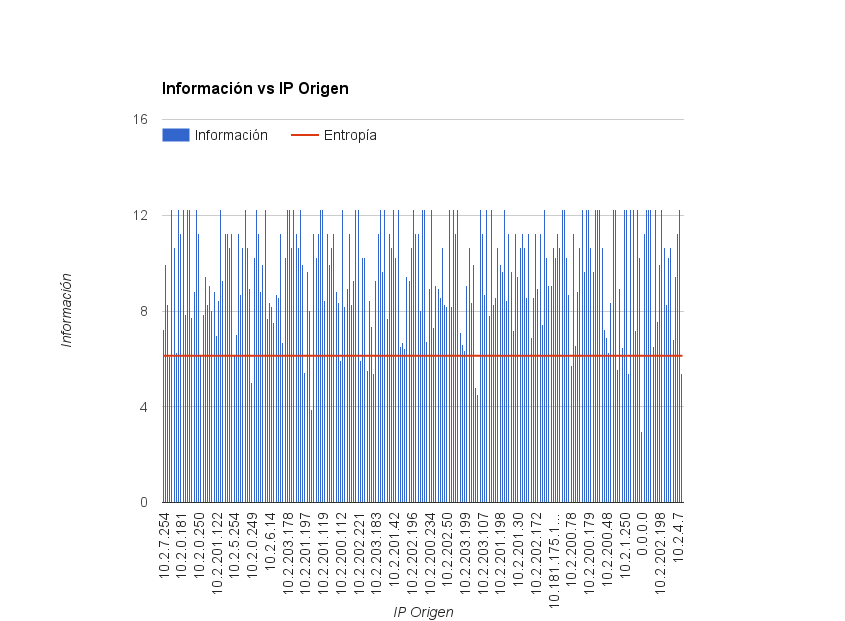
\includegraphics[width=1.1\textwidth]{imagenes/labosDC/ip_informacion.png}
  \caption{Información de los símbolos de la fuente $S_1$}
  \label{fig:ejemplo}
\end{figure}

El nodo que estimamos que era el router una vez más presenta un valor de información inferior a la entropía de la fuente. Sin embargo, en esta red varios nodos presentan un valor de información
inferior a la entropía de la fuente. Quizás éstos nodos también tengan algún rol administrativo dentro de la red pero no lo sabemos con seguridad.

\begin{figure}[H]
  \centering
    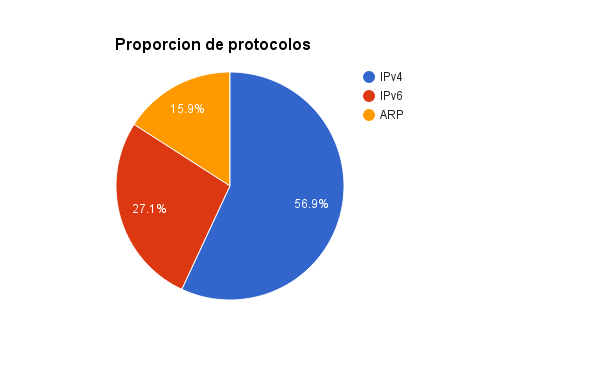
\includegraphics[width=0.7\textwidth]{imagenes/labosDC/proporcion_protocolos.png}
  \caption{Proporción de protocolos observados en el trafico de la red Laboratorios DC}
  \label{fig:ejemplo}
\end{figure}

En esta red en particular podemos observar que el trafico impuesto por ARP es superior al 15\% del trafico total de la red y recordemos que en las anteriores redes analizadas este valor rondaba el 5\% del trafico de la red. Este aumento puede deberse a la gran cantidad de IPs (\textit{host}) que hay en esta red en comparación con las redes anteriores.\\
Al igual que sucedió en las redes anteriores, el protocolo IPv4 es predominante en el trafico de paquetes aunque aquí la presencia de IPv6 es mas notoria.

\begin{figure}[H]
  \centering
    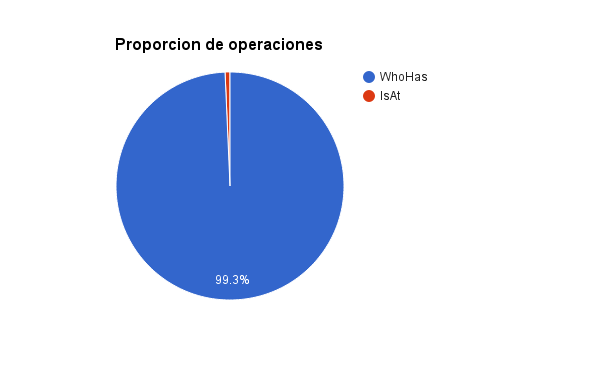
\includegraphics[width=0.9\textwidth]{imagenes/labosDC/proporcion_paquetes_arp.png}
  \caption{Proporción de paquetes who-has vs is-at en red Laboratorios DC}
  \label{fig:ejemplo}
\end{figure}

El digrafo de esta red está simplificado para que entre en las dimensiones de una página ya que al contar con muchas IPs era enorme. La simplificación constó en el filtrado de las aristas con
un peso menor a 20. Los aislados luego de aplicar este filtro fueron retirados del gráfico. El valor 20 fue elegido por ser el menor que conseguía reducir las dimensiones del gráfico lo suficiente
para entrar en una página A4.

\begin{figure}[H]
  \centering
    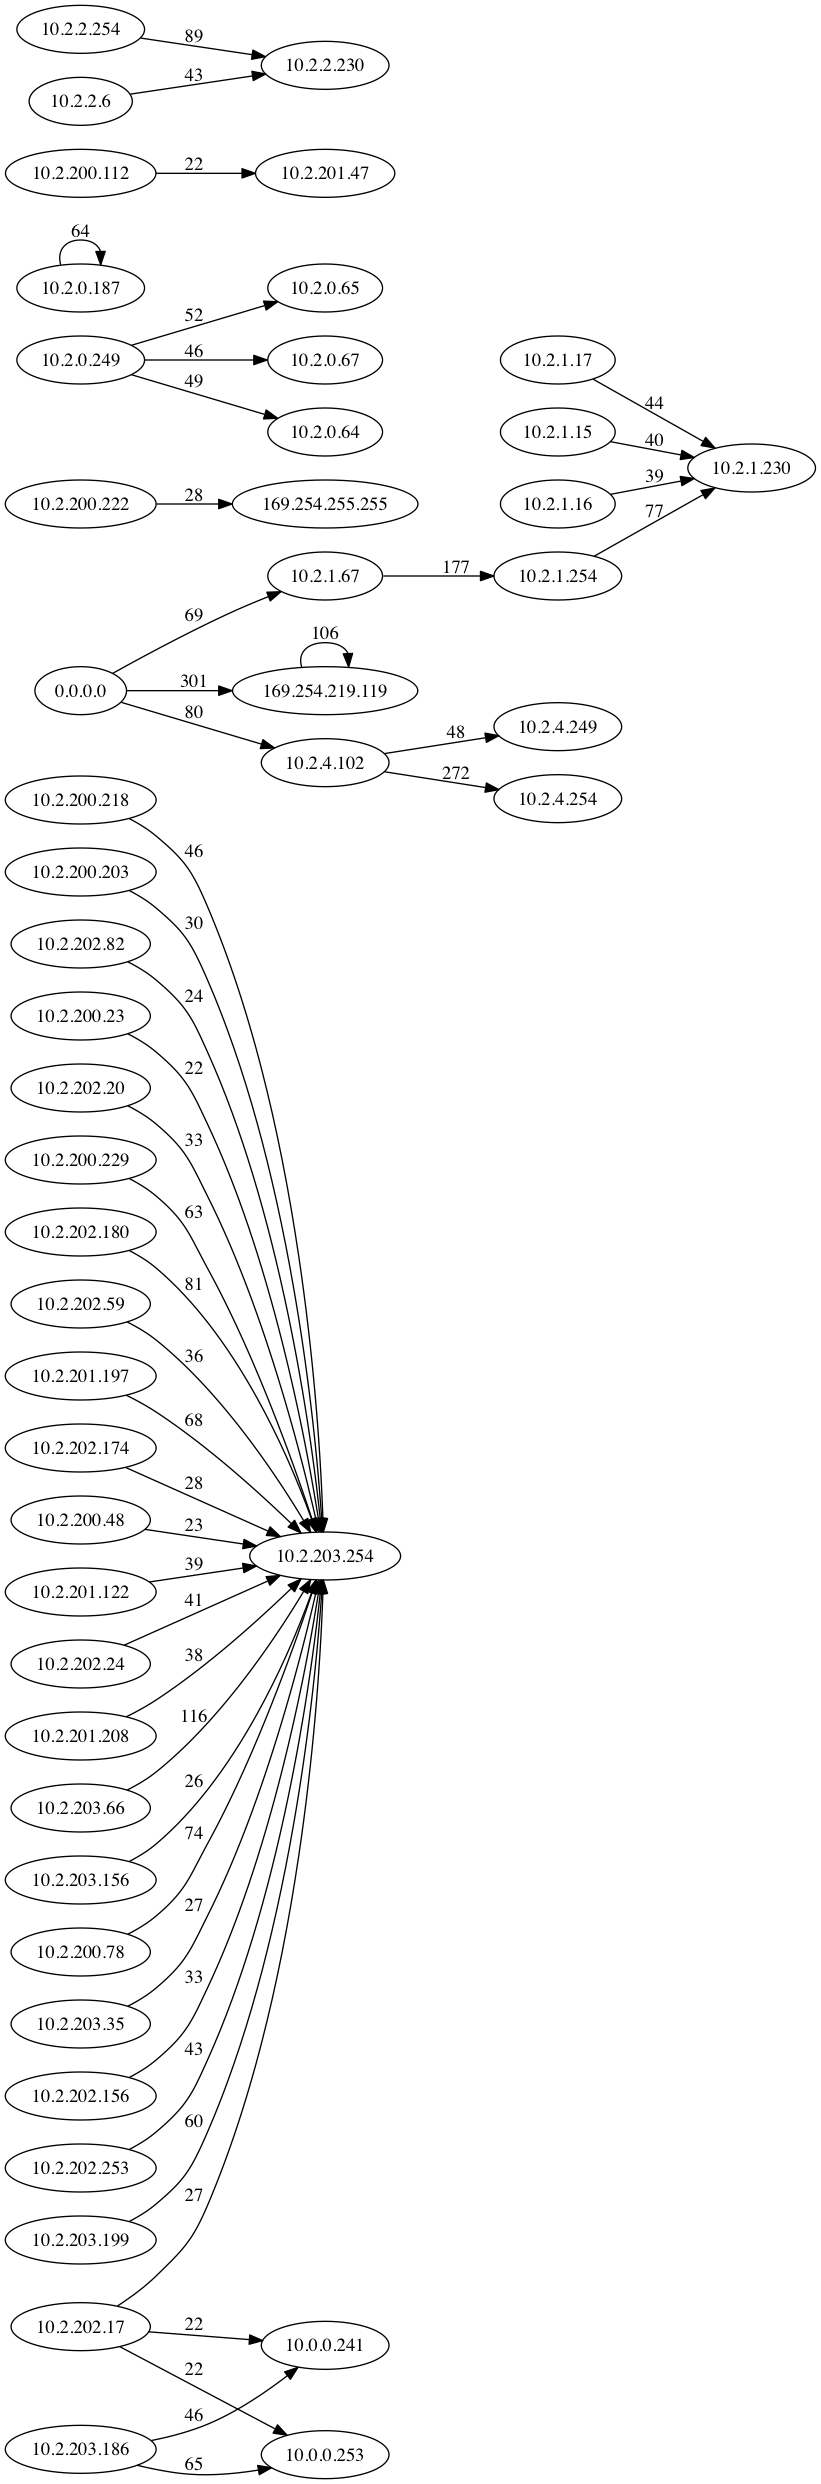
\includegraphics[width=0.48\textwidth]{imagenes/labosDC/digrafo_labosDC.png}
  \caption{Trafico de paquetes ARP entre las IP de la red Laboratorios DC}
  \label{fig:ejemplo}
\end{figure}

En esta red tenemos varios nodos distinguidos, entre ellos:
\begin{itemize}
	\item La IP 0.0.0.0, cuyo propósito lo explicamos en el análisis de la red anterior.
	\item La IP 10.2.203.254, que suponemos es el router de la red, ya que concentra la mayor parte del trafico ARP.
	\item Las IPs en el rango 169.254.0.0/16, que también fue explicado en el análisis de la red anterior.
\end{itemize}

El resto de las direcciones IPs no posee un trafico ARP tan considerable como para distinguirse del resto.\\
También es importante notar que en esta red se da mucho el caso en el que un host envía un paquete ARP \textit{who-has} con su dirección IP como origen y destino. El significado de estos mensajes fue explicado en el análisis de la red Starbucks.

\newpage